\section{zadanie 5}
Zadanie polegało na przetestowaniu funkcji /(rysujNnfx/) przygotowanej na potrzeby wcześniejszego zadania. Testy zostały wykonane na następujących danych wejściowych:
\begin{enumerate}
  \item \(f(x) = e^x; [a, b] = [0, 1], n = 5, 10, 15 \)
  \item \(f(x) = x^2\sin(x); [a, b] = [-1, 1], n = 5, 10, 15 \)
\end{enumerate}

\subsection{Wyniki:}

\begin{figure}[ht]
  \centering
  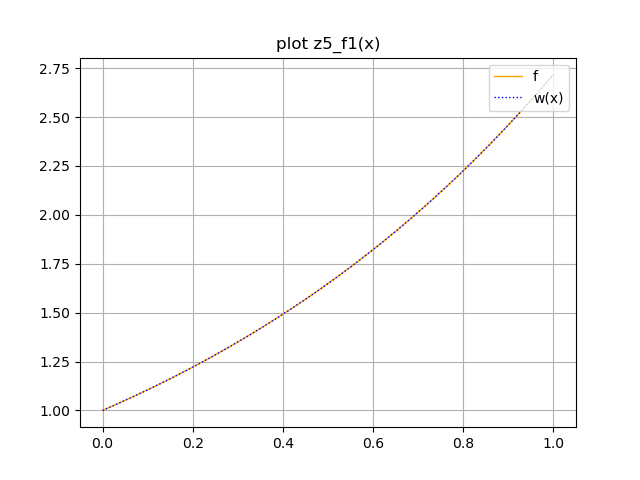
\includegraphics[width=\textwidth]{plot_z5_f1(x)_5.png}
  \caption{Wykresy funkcji \(f(x) = e^x, n = 5\)}
\end{figure}

\begin{figure}[ht]
  \centering
  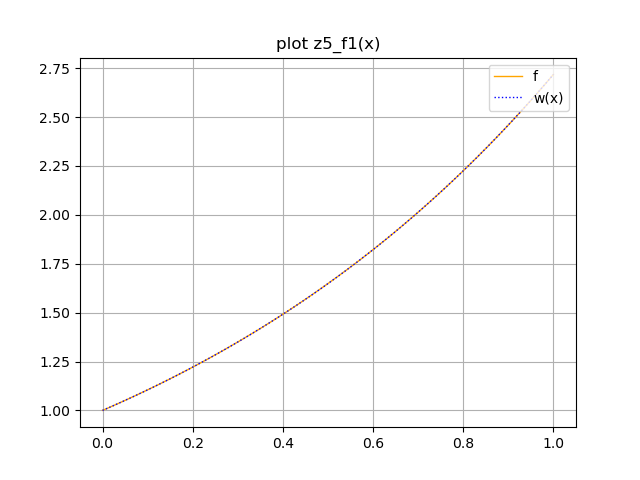
\includegraphics[width=\textwidth]{plot_z5_f1(x)_10.png}
  \caption{Wykresy funkcji \(f(x) = e^x, n = 10\)}
\end{figure}

\begin{figure}[ht]
  \centering
  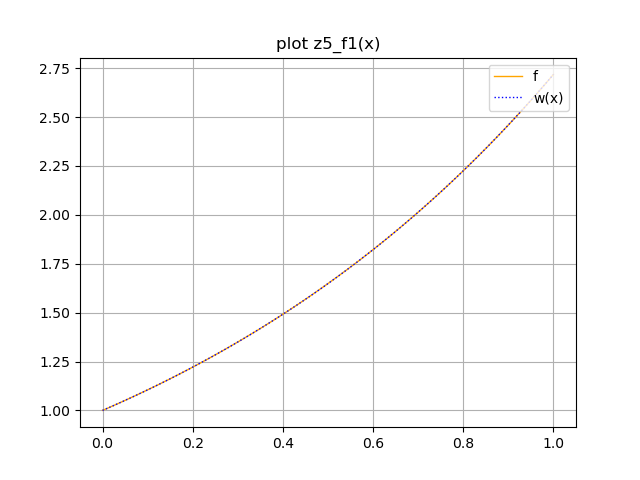
\includegraphics[width=\textwidth]{plot_z5_f1(x)_15.png}
  \caption{Wykresy funkcji \(f(x) = e^x, n = 15\)}
\end{figure}

\begin{figure}[ht]
  \centering
  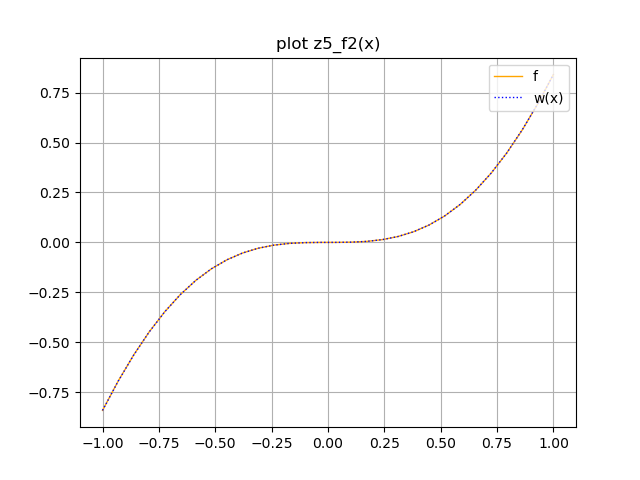
\includegraphics[width=\textwidth]{plot_z5_f2(x)_5.png}
  \caption{Wykresy funkcji \(f(x) = x^2sin(x), n = 5\)}
\end{figure}

\begin{figure}[ht]
  \centering
  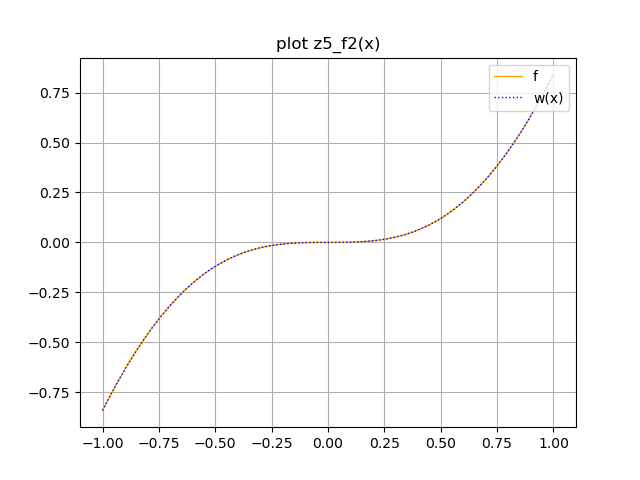
\includegraphics[width=\textwidth]{plot_z5_f2(x)_10.png}
  \caption{Wykresy funkcji \(f(x) = x^2sin(x), n = 10\)}
\end{figure}

\begin{figure}[ht]
  \centering
  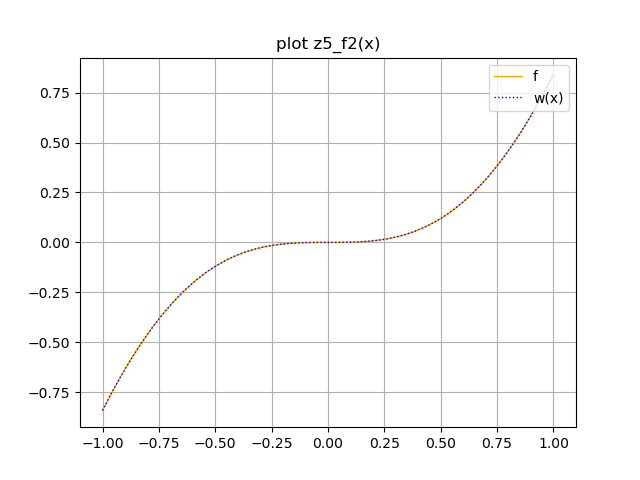
\includegraphics[width=\textwidth]{plot_z5_f2(x)_15.png}
  \caption{Wykresy funkcji \(f(x) = x^2sin(x), n = 15\)}
\end{figure}



\subsection{Wnioski:}
Funkcje wydają się być 'porządne' tj. ich wielomianowe przybliżenie nie odbiega znacząco od spodziewanych rezultatów na zadanych przedziałach.
